%\documentclass[12pt]{scrbook}
%
%\usepackage{tikz}
%\usepackage{minted}
%\usetikzlibrary{decorations.pathreplacing}
%\usetikzlibrary{patterns}
%
%\usepackage{fullpage}
%\usepackage{subfigure}
%\begin{document}
%
%
%Lorem Ipsum is simply dummy text of the printing and typesetting industry. Lorem Ipsum has been the industry's standard dummy text ever since the 1500s, when an unknown printer took a galley of type and scrambled it to make a type specimen book. It has survived not only five centuries, but also the leap into electronic typesetting, remaining essentially unchanged. It was popularised in the 1960s with the release of Letraset sheets containing Lorem Ipsum passages, and more recently with desktop publishing software like Aldus PageMaker including versions of Lorem Ipsum.
%

\begin{figure}
\centering

\subfigure[Upon invocation of the \mintinline{c}{sum()} function, a new stack frame is created which holds
the parameters and local variable.  The parameter variables \mintinline{c}{a} and \mintinline{c}{b}
are \emph{distinct} from the original argument variables \mintinline{c}{n} and \mintinline{c}{m}.]{

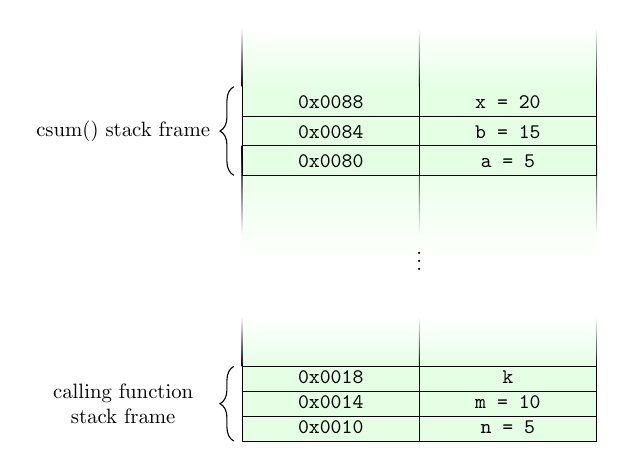
\begin{tikzpicture}[auto,scale=.75,transform shape,every node/.style={text centered}]

%\draw[path fading=north] (0,15.5) -- (0, 18.5);

\draw[fill=green!10!white] (0, 0) rectangle (3, 1.2em);
\node [above] (a1) at (1.5,0) {\texttt{0x0010}};
\draw[fill=green!10!white] (3, 0) rectangle (6, 1.2em);
\node [above] (a2) at (4.5,0) {\texttt{n = 5}};

\draw[fill=green!10!white] (0, 0+1.2em) rectangle (3, 2.4em);
\node [above] (b1) at (1.5,0+1.2em) {\texttt{0x0014}};
\draw[fill=green!10!white] (3, 0+1.2em) rectangle (6, 2.4em);
\node [above] (b2) at (4.5,0+1.2em) {\texttt{m = 10}};

\draw[fill=green!10!white] (0, 0+2.4em) rectangle (3, 3.6em);
\node [above] (b1) at (1.5,0+2.4em) {\texttt{0x0018}};
\draw[fill=green!10!white] (3, 0+2.4em) rectangle (6, 3.6em);
\node [above] (b2) at (4.5,0+2.4em) {\texttt{k}};

\path [top color=white, bottom color=green!10!white] (0,3.625em) rectangle (6,6em);

\fill [top color=white, bottom color=black] (-0.0075,3.6em) rectangle (.02em,6em);
\fill [top color=white, bottom color=black] (5.9925,3.6em) rectangle (6.0075,6em);
\fill [top color=white, bottom color=black] (2.9925,3.6em) rectangle (3.0075,6em);
      
%\draw[top color=white,
%      bottom color=green!10!white]
% (0,3.6em) rectangle (6,6em);
 
%\draw[bottom color=transparent!0,top color=transparent!100] (0,3.6em) -- (0,6em);
%\draw[] (6cm,3.6em) -- (6cm,6em);

%\draw[dashed] (0, 5) -- (6, 5);
%\node [above] (mainvar) at (3,5) {return address, value (\mintinline{c}{0})};
%\draw[dashed] (0, 6) -- (6, 6);
%\node [above] (mainvar2) at (3,6) {local variables \mintinline{c}{n, m, ave}};
\draw [decorate,decoration={brace,amplitude=5pt},xshift=-4pt,yshift=0pt] (0, 0) -- (0, 3.6em) node [text width=3cm,align=center,black,midway,xshift=-.25cm]  {calling function stack frame};


\path [top color=green!10!white, bottom color=white] (0,3) rectangle (6,5);
\fill [top color=black, bottom color=white] (-0.0075,3.5) rectangle (.01,5);
\fill [top color=black, bottom color=white] (2.9925,3.5) rectangle (3.01,5);
\fill [top color=black, bottom color=white] (5.9925,3.5) rectangle (6.01,5);

\draw[fill=green!10!white] (0, 4.5) rectangle (3, 5);
\node [above] (aa1) at (1.5,4.5) {\texttt{0x0080}};
\draw[fill=green!10!white] (3, 4.5) rectangle (6, 5);
\node [above] (aa2) at (4.5,4.5) {\texttt{a = 5}};

\draw[fill=green!10!white] (0, 5) rectangle (3, 5.5);
\node [above] (bb1) at (1.5,5) {\texttt{0x0084}};
\draw[fill=green!10!white] (3, 5) rectangle (6, 5.5);
\node [above] (bb2) at (4.5,5) {\texttt{b = 15}};

\draw[fill=green!10!white] (0, 5.5) rectangle (3, 6);
\node [above] (cc1) at (1.5,5.5) {\texttt{0x0088}};
\draw[fill=green!10!white] (3, 5.5) rectangle (6, 6);
\node [above] (cc2) at (4.5,5.5) {\texttt{x = 20}};

\draw [decorate,decoration={brace,amplitude=5pt},xshift=-4pt,yshift=0pt] (0, 4.5) -- (0, 6) node [text width=3cm,align=center,black,midway,xshift=-.25cm]  {\mintinline{c}{sum()} stack frame};

\node (dots) at (3, 3.15) {$\vdots$};

\path [top color=white, bottom color=green!10!white] (0,6.01) rectangle (6,7);

\fill [top color=white, bottom color=black] (-0.00725,6) rectangle (.0075,7);
\fill [top color=white, bottom color=black] (5.9925,6) rectangle (6.0075,7);
\fill [top color=white, bottom color=black] (2.9925,6) rectangle (3.0075,7);


\end{tikzpicture}
}~~~~\subfigure[The change to the variable \mintinline{c}{a} in the \mintinline{c}{sum()}
function changes the parameter variable, but the original variable \mintinline{c}{n}
is unaffected.]{

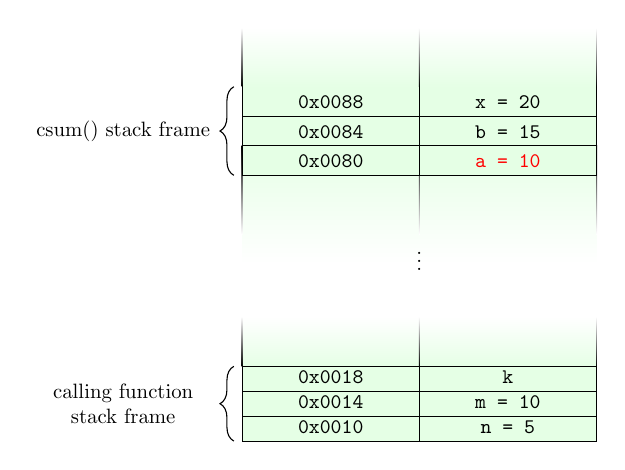
\begin{tikzpicture}[auto,scale=.75,transform shape,every node/.style={text centered}]

%\draw[path fading=north] (0,15.5) -- (0, 18.5);

\draw[fill=green!10!white] (0, 0) rectangle (3, 1.2em);
\node [above] (a1) at (1.5,0) {\texttt{0x0010}};
\draw[fill=green!10!white] (3, 0) rectangle (6, 1.2em);
\node [above] (a2) at (4.5,0) {\texttt{n = 5}};

\draw[fill=green!10!white] (0, 0+1.2em) rectangle (3, 2.4em);
\node [above] (b1) at (1.5,0+1.2em) {\texttt{0x0014}};
\draw[fill=green!10!white] (3, 0+1.2em) rectangle (6, 2.4em);
\node [above] (b2) at (4.5,0+1.2em) {\texttt{m = 10}};

\draw[fill=green!10!white] (0, 0+2.4em) rectangle (3, 3.6em);
\node [above] (b1) at (1.5,0+2.4em) {\texttt{0x0018}};
\draw[fill=green!10!white] (3, 0+2.4em) rectangle (6, 3.6em);
\node [above] (b2) at (4.5,0+2.4em) {\texttt{k}};

\path [top color=white, bottom color=green!10!white] (0,3.625em) rectangle (6,6em);

\fill [top color=white, bottom color=black] (-0.0075,3.6em) rectangle (.02em,6em);
\fill [top color=white, bottom color=black] (5.9925,3.6em) rectangle (6.0075,6em);
\fill [top color=white, bottom color=black] (2.9925,3.6em) rectangle (3.0075,6em);
      
%\draw[top color=white,
%      bottom color=green!10!white]
% (0,3.6em) rectangle (6,6em);
 
%\draw[bottom color=transparent!0,top color=transparent!100] (0,3.6em) -- (0,6em);
%\draw[] (6cm,3.6em) -- (6cm,6em);

%\draw[dashed] (0, 5) -- (6, 5);
%\node [above] (mainvar) at (3,5) {return address, value (\mintinline{c}{0})};
%\draw[dashed] (0, 6) -- (6, 6);
%\node [above] (mainvar2) at (3,6) {local variables \mintinline{c}{n, m, ave}};
\draw [decorate,decoration={brace,amplitude=5pt},xshift=-4pt,yshift=0pt] (0, 0) -- (0, 3.6em) node [text width=3cm,align=center,black,midway,xshift=-.25cm]  {calling function stack frame};


\path [top color=green!10!white, bottom color=white] (0,3) rectangle (6,5);
\fill [top color=black, bottom color=white] (-0.0075,3.5) rectangle (.01,5);
\fill [top color=black, bottom color=white] (2.9925,3.5) rectangle (3.01,5);
\fill [top color=black, bottom color=white] (5.9925,3.5) rectangle (6.01,5);

\draw[fill=green!10!white] (0, 4.5) rectangle (3, 5);
\node [above] (aa1) at (1.5,4.5) {\texttt{0x0080}};
\draw[fill=green!10!white] (3, 4.5) rectangle (6, 5);
\node [above] (aa2) at (4.5,4.5) { \color{red}{\texttt{a = 10}}};

\draw[fill=green!10!white] (0, 5) rectangle (3, 5.5);
\node [above] (bb1) at (1.5,5) {\texttt{0x0084}};
\draw[fill=green!10!white] (3, 5) rectangle (6, 5.5);
\node [above] (bb2) at (4.5,5) {\texttt{b = 15}};

\draw[fill=green!10!white] (0, 5.5) rectangle (3, 6);
\node [above] (cc1) at (1.5,5.5) {\texttt{0x0088}};
\draw[fill=green!10!white] (3, 5.5) rectangle (6, 6);
\node [above] (cc2) at (4.5,5.5) {\texttt{x = 20}};

\draw [decorate,decoration={brace,amplitude=5pt},xshift=-4pt,yshift=0pt] (0, 4.5) -- (0, 6) node [text width=3cm,align=center,black,midway,xshift=-.25cm]  {\mintinline{c}{sum()} stack frame};

\node (dots) at (3, 3.15) {$\vdots$};

\path [top color=white, bottom color=green!10!white] (0,6.01) rectangle (6,7);

\fill [top color=white, bottom color=black] (-0.00725,6) rectangle (.0075,7);
\fill [top color=white, bottom color=black] (5.9925,6) rectangle (6.0075,7);
\fill [top color=white, bottom color=black] (2.9925,6) rectangle (3.0075,7);


\end{tikzpicture}

}

\subfigure[When the \mintinline{c}{sum()} function finishes execution, its stack frame
is removed and the variables \mintinline{c}{a}, \mintinline{c}{b}, and \mintinline{c}{x} are
no longer valid.  The return value 20 is stored in another return value location.]{


\begin{tikzpicture}[auto,scale=.75,transform shape,every node/.style={text centered}]

%\draw[path fading=north] (0,15.5) -- (0, 18.5);

\draw[fill=green!10!white] (0, 0) rectangle (3, 1.2em);
\node [above] (a1) at (1.5,0) {\texttt{0x0010}};
\draw[fill=green!10!white] (3, 0) rectangle (6, 1.2em);
\node [above] (a2) at (4.5,0) {\texttt{n = 5}};

\draw[fill=green!10!white] (0, 0+1.2em) rectangle (3, 2.4em);
\node [above] (b1) at (1.5,0+1.2em) {\texttt{0x0014}};
\draw[fill=green!10!white] (3, 0+1.2em) rectangle (6, 2.4em);
\node [above] (b2) at (4.5,0+1.2em) {\texttt{m = 10}};

\draw[fill=green!10!white] (0, 0+2.4em) rectangle (3, 3.6em);
\node [above] (b1) at (1.5,0+2.4em) {\texttt{0x0018}};
\draw[fill=green!10!white] (3, 0+2.4em) rectangle (6, 3.6em);
\node [above] (b2) at (4.5,0+2.4em) {\color{black}{\texttt{k}}};

\path [top color=white, bottom color=green!10!white] (0,3.625em) rectangle (6,6em);

\fill [top color=white, bottom color=black] (-0.0075,3.6em) rectangle (.02em,6em);
\fill [top color=white, bottom color=black] (5.9925,3.6em) rectangle (6.0075,6em);
\fill [top color=white, bottom color=black] (2.9925,3.6em) rectangle (3.0075,6em);
      
%\draw[top color=white,
%      bottom color=green!10!white]
% (0,3.6em) rectangle (6,6em);
 
%\draw[bottom color=transparent!0,top color=transparent!100] (0,3.6em) -- (0,6em);
%\draw[] (6cm,3.6em) -- (6cm,6em);

%\draw[dashed] (0, 5) -- (6, 5);
%\node [above] (mainvar) at (3,5) {return address, value (\mintinline{c}{0})};
%\draw[dashed] (0, 6) -- (6, 6);
%\node [above] (mainvar2) at (3,6) {local variables \mintinline{c}{n, m, ave}};
\draw [decorate,decoration={brace,amplitude=5pt},xshift=-4pt,yshift=0pt] (0, 0) -- (0, 3.6em) node [text width=3cm,align=center,black,midway,xshift=-.25cm]  {calling function stack frame};


\path [top color=green!10!white, bottom color=white] (0,3) rectangle (6,5);
\fill [top color=black, bottom color=white] (-0.0075,3.5) rectangle (.01,5);
\fill [top color=black, bottom color=white] (2.9925,3.5) rectangle (3.01,5);
\fill [top color=black, bottom color=white] (5.9925,3.5) rectangle (6.01,5);

\draw[fill=green!10!white] (0, 4.5) rectangle (3, 5);
\node [above] (aa1) at (1.5,4.5) {\texttt{0x0080}};
\draw[fill=green!10!white] (3, 4.5) rectangle (6, 5);
\node [above] (aa2) at (4.5,4.5) {\texttt{a = 10}};

\draw[fill=green!10!white] (0, 5) rectangle (3, 5.5);
\node [above] (bb1) at (1.5,5) {\texttt{0x0084}};
\draw[fill=green!10!white] (3, 5) rectangle (6, 5.5);
\node [above] (bb2) at (4.5,5) {\texttt{b = 15}};

\draw[fill=green!10!white] (0, 5.5) rectangle (3, 6);
\node [above] (cc1) at (1.5,5.5) {\texttt{0x0088}};
\draw[fill=green!10!white] (3, 5.5) rectangle (6, 6);
\node [above] (cc2) at (4.5,5.5) {\texttt{x = 20}};

%cross outs: 
\draw[pattern=north west lines, pattern color=blue!50!white] (0,4.5) rectangle (6,6);


\draw [decorate,decoration={brace,amplitude=5pt},xshift=-4pt,yshift=0pt] (0, 4.5) -- (0, 6) node [text width=3cm,align=center,black,midway,xshift=-.25cm]  {\mintinline{c}{sum()} stack frame};

\node (dots) at (3, 3.15) {$\vdots$};

\path [top color=white, bottom color=green!10!white] (0,6.01) rectangle (6,7);

\fill [top color=white, bottom color=black] (-0.00725,6) rectangle (.0075,7);
\fill [top color=white, bottom color=black] (5.9925,6) rectangle (6.0075,7);
\fill [top color=white, bottom color=black] (2.9925,6) rectangle (3.0075,7);


\end{tikzpicture}

}~~~~~\subfigure[The returned value is stored in the variable \mintinline{c}{k} and
the variable \mintinline{c}{n} retains its original value.]{


\begin{tikzpicture}[auto,scale=.75,transform shape,every node/.style={text centered}]

%\draw[path fading=north] (0,15.5) -- (0, 18.5);

\draw[fill=green!10!white] (0, 0) rectangle (3, 1.2em);
\node [above] (a1) at (1.5,0) {\texttt{0x0010}};
\draw[fill=green!10!white] (3, 0) rectangle (6, 1.2em);
\node [above] (a2) at (4.5,0) {\texttt{n = 5}};

\draw[fill=green!10!white] (0, 0+1.2em) rectangle (3, 2.4em);
\node [above] (b1) at (1.5,0+1.2em) {\texttt{0x0014}};
\draw[fill=green!10!white] (3, 0+1.2em) rectangle (6, 2.4em);
\node [above] (b2) at (4.5,0+1.2em) {\texttt{m = 10}};

\draw[fill=green!10!white] (0, 0+2.4em) rectangle (3, 3.6em);
\node [above] (b1) at (1.5,0+2.4em) {\texttt{0x0018}};
\draw[fill=green!10!white] (3, 0+2.4em) rectangle (6, 3.6em);
\node [above] (b2) at (4.5,0+2.4em) {\color{red}{\texttt{k = 20}}};

\path [top color=white, bottom color=green!10!white] (0,3.625em) rectangle (6,6em);

\fill [top color=white, bottom color=black] (-0.0075,3.6em) rectangle (.02em,6em);
\fill [top color=white, bottom color=black] (5.9925,3.6em) rectangle (6.0075,6em);
\fill [top color=white, bottom color=black] (2.9925,3.6em) rectangle (3.0075,6em);
      
%\draw[top color=white,
%      bottom color=green!10!white]
% (0,3.6em) rectangle (6,6em);
 
%\draw[bottom color=transparent!0,top color=transparent!100] (0,3.6em) -- (0,6em);
%\draw[] (6cm,3.6em) -- (6cm,6em);

%\draw[dashed] (0, 5) -- (6, 5);
%\node [above] (mainvar) at (3,5) {return address, value (\mintinline{c}{0})};
%\draw[dashed] (0, 6) -- (6, 6);
%\node [above] (mainvar2) at (3,6) {local variables \mintinline{c}{n, m, ave}};
\draw [decorate,decoration={brace,amplitude=5pt},xshift=-4pt,yshift=0pt] (0, 0) -- (0, 3.6em) node [text width=3cm,align=center,black,midway,xshift=-.25cm]  {calling function stack frame};


\path [top color=green!10!white, bottom color=white] (0,3) rectangle (6,5);
\fill [top color=black, bottom color=white] (-0.0075,3.5) rectangle (.01,5);
\fill [top color=black, bottom color=white] (2.9925,3.5) rectangle (3.01,5);
\fill [top color=black, bottom color=white] (5.9925,3.5) rectangle (6.01,5);

\draw[fill=green!10!white] (0, 4.5) rectangle (3, 5);
\node [above] (aa1) at (1.5,4.5) {\texttt{0x0080}};
\draw[fill=green!10!white] (3, 4.5) rectangle (6, 5);
\node [above] (aa2) at (4.5,4.5) {\texttt{a = 10}};

\draw[fill=green!10!white] (0, 5) rectangle (3, 5.5);
\node [above] (bb1) at (1.5,5) {\texttt{0x0084}};
\draw[fill=green!10!white] (3, 5) rectangle (6, 5.5);
\node [above] (bb2) at (4.5,5) {\texttt{b = 15}};

\draw[fill=green!10!white] (0, 5.5) rectangle (3, 6);
\node [above] (cc1) at (1.5,5.5) {\texttt{0x0088}};
\draw[fill=green!10!white] (3, 5.5) rectangle (6, 6);
\node [above] (cc2) at (4.5,5.5) {\texttt{x = 20}};

%cross outs: 
\draw[pattern=north west lines, pattern color=blue!50!white] (0,4.5) rectangle (6,6);


\draw [decorate,decoration={brace,amplitude=5pt},xshift=-4pt,yshift=0pt] (0, 4.5) -- (0, 6) node [text width=3cm,align=center,black,midway,xshift=-.25cm]  {\mintinline{c}{sum()} stack frame};

\node (dots) at (3, 3.15) {$\vdots$};

\path [top color=white, bottom color=green!10!white] (0,6.01) rectangle (6,7);

\fill [top color=white, bottom color=black] (-0.00725,6) rectangle (.0075,7);
\fill [top color=white, bottom color=black] (5.9925,6) rectangle (6.0075,7);
\fill [top color=white, bottom color=black] (2.9925,6) rectangle (3.0075,7);


\end{tikzpicture}

}

\caption[Demonstration of Pass By Value]{Demonstration of Pass By Value.  Passing variables
by value means that \emph{copies} of the values stored in the variables are provided to the 
function.  Changes to parameter variables do not affect the original variables.}
\label{figure:PassByValue}

\end{figure}




%\end{document}
